\chapter{Validation results for the thermal solver} \label{ch:val_therm_solver}

This chapter provides validation results for the thermal solver developed in this work.
The appropriate examples are sourced from \cite{DINEN1991_1_2}  - Prüfung und  Validierung von Rechenprogramm für Brand\-schutz\-nach\-weise mittels allgemeiner Rechenverfahren  and the linear thermo-elastic test in the \cite{NAFEMSbenchmarks}.
They include thermal effects such as variable conductivity, heat convection and radiation at the boundary.
The numerical solutions are obtained using the thermal solver in LINKS, employing TRI3, TRI6, QUAD4, QUAD8 elements, in two-dimensions, and TETRA4 and TETRA10 elements in three-dimensions.
No convergence study was performed, however the mesh size was chosen small enough so that assuming convergence of the FEM solution is reasonable.
Moreover the good agreement with reference solutions supports this assumption.

\section{Validation example 1 - DIN EN 1991-1-2/NA:2010-12: Anhang CC - Prüfung und Validierung von Rechenprogramm für Brandschutznachweise mittels allgemeiner Rechenverfahren - Beispiel 1)}

\subsection{Description}

The geometry examined is a square plate with side length equal to \SI{1}{\meter}, as shown in Figure~\ref{fig:din_example_1_plate}.
The boundary conditions considered are as follows: the left, upper and right edges are assumed to be adiabatic.
At the lower edge there is heat transfer by convection with a heat convection coefficient \(h_c\) equation to \SI{1}{\watt\meter^{-2}\kelvin^{-1}} and an environment temperature equal to \SI{0}{\celsius} (see Equation~\ref{eq:heat_convection}).
The initial temperature for the entire plate is \SI{1000}{\celsius}.
Reference values for the temperature at the middle of the upper edge are supplied to determine performance.
The relevant properties of the material making up the plate are its conductivity \(k\), equal to \SI{1}{\watt\meter^{-1}\kelvin^{-1}}, its specific heat \(c_p\), equal to \SI{1}{\joule\kilo\gram^{-1}\kelvin^{-1}}, and its density \(\rho\), set equal to \SI{1000}{\kilo\gram\meter^{-3}}.
Table~\ref{tab:din_example_1_description} summarizes all the information regarding initial and boundary conditions, geometry and material properties.

\begin{figure}[htbp]
  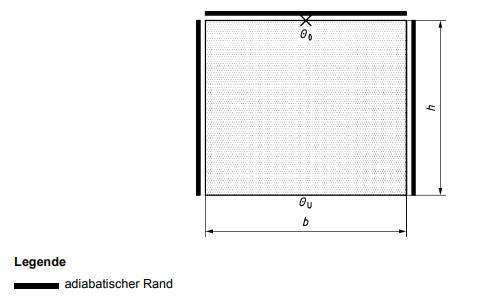
\includegraphics[width=0.8\textwidth]{din_example_1_plate.png}
  \caption{Geometry and boundary conditions considered in the validation example 1 \citep{DINEN1991_1_2}.}
\label{fig:din_example_1_plate}
\end{figure}

\begin{table}[htbp]
  \centering
  \caption{Material properties, and initial and boundary conditions for validation example 1.}
  \label{tab:din_example_1_description}
  \begin{tabular}{lccS[exponent-mode=engineering]}
  \multicolumn{3}{c}{Material Properties} & {\vphantom{\Big |}Effective value}\\
  \hline\hline
  \vphantom{\Big |}Conductivity & \(k\) & (\si{\watt\meter^{-1}\kelvin^{-1}}) & 1\\
  \vphantom{\Big |}Specific heat & \(c_p\) & (\si{\joule\per\kilo\gram\per\kelvin}) & 1\\
  \vphantom{\Big |}Density & \(\rho\) & (\si{\kilo\gram\per\meter^{3}}) & 1000\\
  \hline
  \multicolumn{3}{c}{Boundary Conditions\vphantom{\Big |}} & \\\hline
  \vphantom{\Big |}Dimensions & \(h\), \(b\) & (\si{\meter}) & 1\\
  \vphantom{\Big |}Heat convection coefficient & \(h_c\) & (\si{\watt\per\meter^2\per\kelvin}) & 1\\
  \hline
  \multicolumn{3}{c}{Initial Conditions\vphantom{\Big |}} & \\\hline
  \vphantom{\Big |}Ambient temperature & \(T_\infty\) & (\si{\celsius}) & 0\\
  \vphantom{\Big |}Temperature in cross-section & \(T_0\) & (\si{\celsius}) & 1000\\
  \hline
  \multicolumn{3}{c}{Reference value \vphantom{\Big |}} & \\\hline
  \vphantom{\Big |}Temperature \(T\) at point \(X\) & (\si{\celsius}) & \\
  \hline\hline
  \end{tabular}
\end{table}

\subsection{Results}

The numerical solutions obtained using FEM are presented in Table~\ref{tab:dim_example_1_comparison_table}, as well as, the reference values and the corresponding relative difference.
Figure~\ref{fig:dim_example_1_comparison} presents the same results in graphical form.
It can seen that that agreement between the numerical results and the reference solutions is very good, with relative error always smaller than \num{0.02}\%.
\cite{} recomends a relative difference \(\pm 1\%\) and an absolute difference \(\pm \SI{5}{\celsius}\).
Figure~\ref{fig:DIN_example_1_TRI3} shows different time instants of the numerical solution using TRI3 elements.
The evolution of the temperature field depicted seems reasonable given the description of the problem.

\begin{table}
  \caption{Reference and computed values for \(T_0\) concerning the validation example 1.}
  \label{tab:dim_example_1_comparison_table}
  \centering
  \begin{tabular}{SSc
      S[round-mode=places, round-precision=4]
      S[exponent-mode=scientific, round-mode=places, round-precision=2]}
   {Time (\si{\second})} & {\makecell{Reference value\\\(T_0\) (\si{\celsius})}} & \makecell{Element\\Type} & {\makecell{Computed value\\\(T'_0\) (\si{\celsius})}} & {\makecell{Relative difference\\\(\varepsilon\) (\(\%\))}} \\\hline\hline
   {\multirow{4}{*}{ 0 }} & {\multirow{4}{*}{ 1000.0 }} & TRI3  & 1000.0 & 0.0\\
   &  & TRI6 & 1000.0 & 0.0\\
   &  & QUAD4 & 1000.0 & 0.0\\
   &  & QUAD8 & 1000.0 & 0.0\\\hline
   {\multirow{4}{*}{ 60 }} & {\multirow{4}{*}{ 999.3 }} & TRI3  & 999.3436 & 0.004363054137904846\\
   &  & TRI6 & 999.2821 & 0.0017912538777084478\\
   &  & QUAD4 & 999.3434 & 0.004343040128091629\\
   &  & QUAD8 & 999.2821 & 0.0017912538777084478\\\hline
   {\multirow{4}{*}{ 300 }} & {\multirow{4}{*}{ 891.8 }} & TRI3  & 891.9305 & 0.014633325857826568\\
   &  & TRI6 & 891.7957 & 0.00048217089032785303\\
   &  & QUAD4 & 891.9308 & 0.01466696568737632\\
   &  & QUAD8 & 891.7957 & 0.00048217089032785303\\\hline
   {\multirow{4}{*}{ 600 }} & {\multirow{4}{*}{ 717.7 }} & TRI3  & 717.7402 & 0.005601226139043251\\
   &  & TRI6 & 717.6768 & 0.0032325484185715533\\
   &  & QUAD4 & 717.7403 & 0.005615159537411453\\
   &  & QUAD8 & 717.6768 & 0.0032325484185715533\\\hline
   {\multirow{4}{*}{ 900 }} & {\multirow{4}{*}{ 574.9 }} & TRI3  & 574.9004 & 6.957731779670875e-05\\
   &  & TRI6 & 574.8708 & 0.005079144198981763\\
   &  & QUAD4 & 574.9005 & 8.697164724094218e-05\\
   &  & QUAD8 & 574.8708 & 0.005079144198981763\\\hline
   {\multirow{4}{*}{ 1200 }} & {\multirow{4}{*}{ 460.4 }} & TRI3  & 460.4098 & 0.0021285838401479385\\
   &  & TRI6 & 460.4019 & 0.00041268462207529364\\
   &  & QUAD4 & 460.4098 & 0.0021285838401479385\\
   &  & QUAD8 & 460.4019 & 0.00041268462207529364\\\hline
   {\multirow{4}{*}{ 1500 }} & {\multirow{4}{*}{ 368.7 }} & TRI3  & 368.7175 & 0.004746406292374311\\
   &  & TRI6 & 368.7238 & 0.006455112557633379\\
   &  & QUAD4 & 368.7175 & 0.004746406292374311\\
   &  & QUAD8 & 368.7238 & 0.006455112557633379\\\hline
   {\multirow{4}{*}{ 1800 }} & {\multirow{4}{*}{ 295.3 }} & TRI3  & 295.286 & 0.004740941415513039\\
   &  & TRI6 & 295.3011 & 0.0003725025397927851\\
   &  & QUAD4 & 295.286 & 0.004740941415513039\\
   &  & QUAD8 & 295.3011 & 0.0003725025397927851\\
  \hline\hline
  \end{tabular}
\end{table}

% \begin{table}
%   \caption{Reference and computed values for \(T_0\) concerning the validation example 1 using TRI3 elements.}
%   \label{tab:dim_example_1_comparison_table}
%   \centering
%   \begin{tabular}{SS
%       S
%       S[exponent-mode=scientific, round-mode=places, round-precision=2]
%       c}
%   {Time (\si{\second})} & {\makecell{Reference value\\\(T_0\) (\si{\celsius})}} & {\makecell{Computed value\\\(T'_0\) (\si{\celsius})}} & {\makecell{Relative difference\\\(\varepsilon\) (\(\%\))}} & \makecell{Acceptable\\ difference \\according to \cite{}}\\\hline\hline
%   0 & 1000.0 & 1000.0 & 0.0 & \multirow{8}{*}{\makecell{\(\pm 1\%\)\\and\\\(\pm \SI{5.0}{\kelvin}\)}}\\
%   60 & 999.3 & 999.3436 & 0.004363054137904846 & \\
%   300 & 891.8 & 891.9305 & 0.014633325857826568 & \\
%   600 & 717.7 & 717.7402 & 0.005601226139043251 & \\
%   900 & 574.9 & 574.9004 & 6.957731779670875e-05 & \\
%   1200 & 460.4 & 460.4098 & 0.0021285838401479385 & \\
%   1500 & 368.7 & 368.7175 & 0.004746406292374311 & \\
%   1800 & 295.3 & 295.286 & 0.004740941415513039 & \\
%   \hline\hline
%   \end{tabular}
% \end{table}

\begin{figure}
   \centering
     \subfloat[][]{ 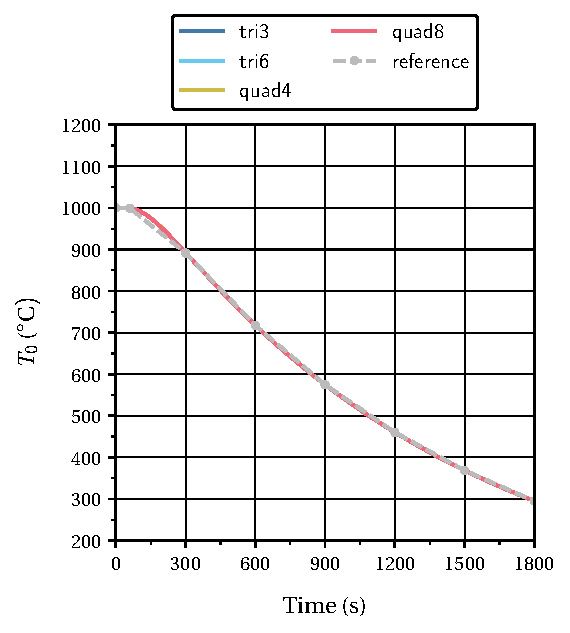
\includegraphics[width=0.5\columnwidth]{example_1_comparison_temp_ref_pt.pdf}
            \label{fig:example_1_comparison_temp_ref_pt}}
     \subfloat[][]{
    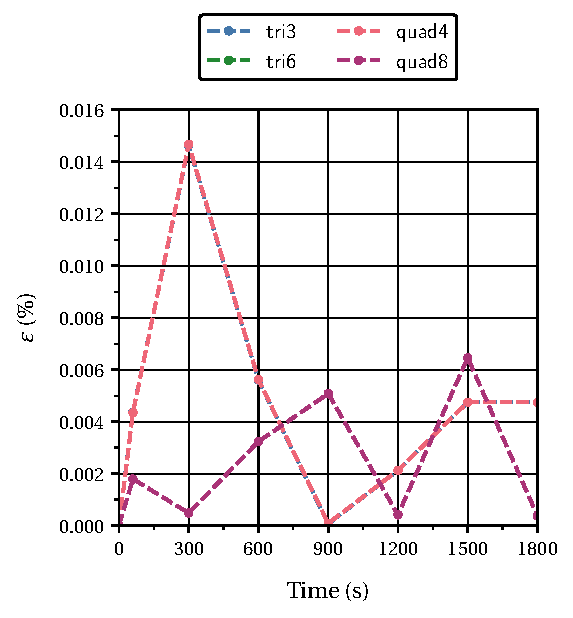
\includegraphics[width=0.5\columnwidth]{example_1_comparison_relative_error.pdf}
            \label{fig:example_1_comparison_relative_error}}
    \caption{Numerical results for the validation example 1. (a) Temperature values at \(X\) as a function of time. (b) Relative error in percentage as function of time.}
    \label{fig:dim_example_1_comparison}
\end{figure}

\begin{figure}
   \centering
     \subfloat[][$t=\SI{60}{\second}$]{ 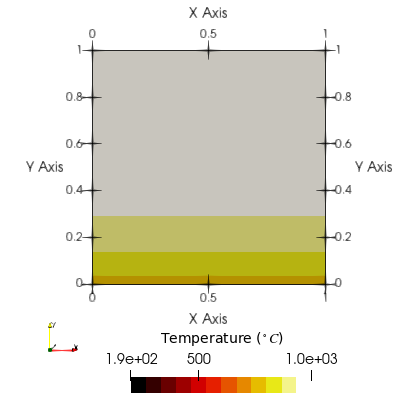
\includegraphics[width=0.5\columnwidth]{DIN_example_1_TRI3_t_60.png}
            \label{fig:DIN_example_1_TRI3_t_60}}
     \subfloat[][$t=\SI{600}{\second}$]{ 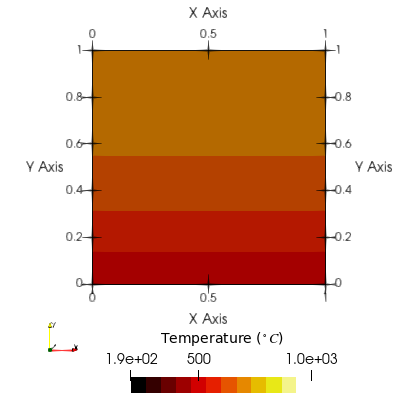
\includegraphics[width=0.5\columnwidth]{DIN_example_1_TRI3_t_600.png}
            \label{fig:DIN_example_1_TRI3_t_60}}\\
     \subfloat[][$t=\SI{1200}{\second}$]{
    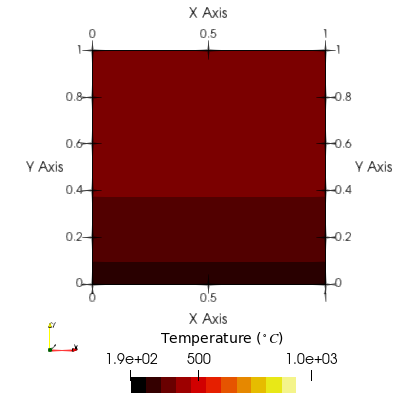
\includegraphics[width=0.5\columnwidth]{DIN_example_1_TRI3_t_1200.png}
            \label{fig:DIN_example_1_TRI3_t_60}}
     \subfloat[][$t=\SI{1800}{\second}$]{
    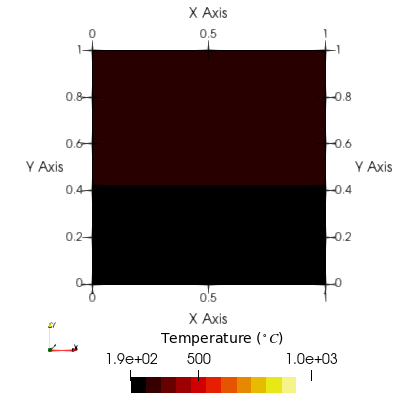
\includegraphics[width=0.5\columnwidth]{DIN_example_1_TRI3_t_1800.png}
            \label{fig:DIN_example_1_TRI3_t_60}}
    \caption{Numerical results regarding the evolution of the temperature distribution for the validation example 1 using a TRI3 mesh.}
    \label{fig:DIN_example_1_TRI3}
\end{figure}

\section{Validation example 2 - DIN EN 1991-1-2/NA:2010-12: Anhang CC - Prüfung und Validierung von Rechenprogramm für Brandschutznachweise mittels allgemeiner Rechenverfahren - Beispiel 2)}

\subsection{Description}

The geometry examined is a square plate with side length equal to \SI{0.2}{\meter}, as shown in Figure~\ref{fig:din_example_2_plate}.
There is heat transfer by convection along all the edges with a heat convection coefficient \(h_c\) equation to \SI{10}{\watt\meter^{-2}\kelvin^{-1}} and an environment temperature equal to \SI{1000}{\celsius} (see Equation~\ref{eq:heat_convection}).
Thre is also heat transfer through radition, with the emissivity \(\varepsilon_\text{res}\) equal to 0.8.
The initial temperature for the entire plate is \SI{0}{\celsius}.
Reference values for the temperature in the middle of the plate are supplied to determine performance.
The relevant properties of the material making up the plate are its conductivity \(k\), which follows a linear behavior (see Table~\ref{tab:din_example_2_description}), its specific heat \(c_p\), equal to \SI{1000}{\joule\kilo\gram^{-1}\kelvin^{-1}}, and its density \(\rho\), set equal to \SI{2400}{\kilo\gram\meter^{-3}}.
Table~\ref{tab:din_example_2_description} summarizes all the information regarding initial and boundary conditions, geometry and material properties.

\begin{figure}
  \centering
  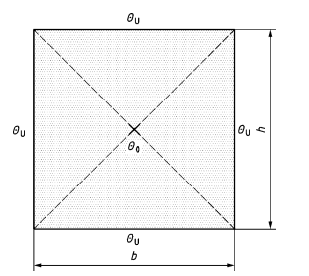
\includegraphics[width=0.55\textwidth]{din_example_2_plate.png}
  \caption{Geometry and boundary conditions considered in the validation example 2. \citep{DINEN1991_1_2}}
\label{fig:din_example_2_plate}
\end{figure}

\begin{table}
  \centering
  \caption{Material properties, and initial and boundary conditions for validation example 2.}
  \label{tab:din_example_2_description}
  \begin{tabular}{lccSS}
  \multicolumn{3}{c}{Material Properties} & \multicolumn{2}{c}{\vphantom{\Big |}Effective value}\\
  \hline\hline
  \multirow{4}{*}{\makecell{Conductivity \\(Linear behavior)}} &  \multirow{4}{*}{\(k\)} & \multirow{4}{*}{(\si{\watt\per\meter\per\kelvin})} & {\(T\)} & {\(\lambda(T)\)}\\\cline{4-5}
  & & & 0 & 1.5\\
  & & & 200 & 0.7\\
  & & & 1000 & 0.5\\
  \vphantom{\Big |} Specific heat & \(c_p\) & (\si{\joule\per\kilo\gram\per\kelvin}) & \multicolumn{2}{c}{1000}\\
  \vphantom{\Big |} Density & \(\rho\) & (\si{\kilo\gram\per\meter^{3}}) & \multicolumn{2}{c}{2400}\\
  \hline
  \multicolumn{3}{c}{Boundary Conditions\vphantom{\Big |}} & \\\hline
  \vphantom{\Big |}Dimensions & \(h\), \(b\) & (\si{\meter}) & \multicolumn{2}{c}{0.2}\\
  \vphantom{\Big |}Heat convection coefficient & \(h_c\) & (\si{\watt\per\meter^2\per\kelvin}) & \multicolumn{2}{c}{10}\\
  \vphantom{\Big |}Emissivity & \(\varepsilon_\text{res}\) &  & \multicolumn{2}{c}{0.8}\\
  \hline
  \multicolumn{3}{c}{Initial Conditions\vphantom{\Big |}} & \\\hline
  \vphantom{\Big |}Ambient temperature & \(T_\infty\) & (\si{\celsius}) & \multicolumn{2}{c}{1000}\\
  \vphantom{\Big |}Temperature in cross-section & \(T_0\) & (\si{\celsius}) & \multicolumn{2}{c}{0}\\
  \hline
  \multicolumn{3}{c}{Reference value \vphantom{\Big |}} & \\\hline
  \vphantom{\Big |}Temperature \(T_0\) in point \(X\) & & (\si{\celsius}) & \\
  \hline\hline
  \end{tabular}
\end{table}

\subsection{Results}

The numerical solutions obtained using FEM are presented in Table~\ref{tab:dim_example_2_comparison_table}, as well as, the reference values and the corresponding relative difference.
Figure~\ref{fig:dim_example_2_comparison} presents the same results in graphical form.
\cite{} recomends for \(t\leq \SI{60}{\minute}\) an absolute difference smaller than \(\pm \SI{5}{\celsius}\), and for \(t>\SI{60}{\minute}\), a relative difference smaller than \(\pm 2\%\).
It can be seen that that agreement between the numerical results and the reference solutions is acceptable.
For \(t\leq \SI{60}{\minute}\) the linear elements do not satisfy the recomendation set forth by \cite{}.
Otherwise the requirements are completly fullfiled.
Figure~\ref{fig:DIN_example_2_TRI3} shows different time instants of the numerical solution using TRI3 elements.
The evolution of the temperature field depicted seems reasonable given the description of the problem.

\begin{table}
  \caption{Reference and computed values for \(T_0\) concerning the validation example 2.}
  \label{tab:dim_example_2_comparison_table}
  \centering
  \begin{tabular}{SSc
      S[round-mode=places, round-precision=4]
      S[exponent-mode=scientific, round-mode=places, round-precision=2]}
   {Time (\si{\minute})} & {\makecell{Reference value\\\(T_0\) (\si{\celsius})}} & \makecell{Element\\Type} & {\makecell{Computed value\\\(T'_0\) (\si{\celsius})}} & {\makecell{Relative difference\\\(\varepsilon\) (\(\%\))}} \\\hline\hline
   {\multirow{4}{*}{ 0 }} & {\multirow{4}{*}{ 0.0 }} & TRI3  & 0.0 & 0.0\\
   &  & TRI6 & 0.0 & 0.0\\
   &  & QUAD4 & 0.0 & 0.0\\
   &  & QUAD8 & 0.0 & 0.0\\\hline
   {\multirow{4}{*}{ 30 }} & {\multirow{4}{*}{ 36.9 }} & TRI3  & 29.73116 & 19.427750677506772\\
   &  & TRI6 & 33.59058 & 8.96861788617885\\
   &  & QUAD4 & 30.42481 & 17.547940379403787\\
   &  & QUAD8 & 33.85025 & 8.26490514905148\\\hline
   {\multirow{4}{*}{ 60 }} & {\multirow{4}{*}{ 137.4 }} & TRI3  & 130.0251 & 5.367467248908294\\
   &  & TRI6 & 133.7875 & 2.629184861717621\\
   &  & QUAD4 & 131.0145 & 4.6473799126637605\\
   &  & QUAD8 & 133.8905 & 2.554221251819507\\\hline
   {\multirow{4}{*}{ 90 }} & {\multirow{4}{*}{ 244.6 }} & TRI3  & 240.0627 & 1.854987735077673\\
   &  & TRI6 & 242.8709 & 0.7069092395748112\\
   &  & QUAD4 & 240.404 & 1.7154538021259191\\
   &  & QUAD8 & 242.95 & 0.6745707277187268\\\hline
   {\multirow{4}{*}{ 120 }} & {\multirow{4}{*}{ 361.1 }} & TRI3  & 362.2362 & 0.3146496815286552\\
   &  & TRI6 & 363.4852 & 0.6605372472999163\\
   &  & QUAD4 & 361.9427 & 0.2333702575463803\\
   &  & QUAD8 & 363.5435 & 0.6766823594572062\\\hline
   {\multirow{4}{*}{ 150}} & {\multirow{4}{*}{ 466.2 }} & TRI3  & 470.0065 & 0.8164950664950725\\
   &  & TRI6 & 470.2503 & 0.8687902187902173\\
   &  & QUAD4 & 469.3439 & 0.674367224367231\\
   &  & QUAD8 & 470.2947 & 0.8783140283140259\\\hline
   {\multirow{4}{*}{ 180 }} & {\multirow{4}{*}{ 554.8 }} & TRI3  & 560.5277 & 1.0323900504686423\\
   &  & TRI6 & 560.1557 & 0.9653388608507697\\
   &  & QUAD4 & 559.6558 & 0.875234318673404\\
   &  & QUAD8 & 560.1907 & 0.9716474405191129\\
  \hline\hline
  \end{tabular}
\end{table}

% \begin{table}
%   \caption{Reference and computed values for \(T_0\) concerning the validation example 1 using TRI3 elements.}
%   \label{tab:dim_example_1_comparison_table}
%   \centering
%   \begin{tabular}{SS
%       S
%       S[exponent-mode=scientific, round-mode=places, round-precision=2]
%       c}
%   {Time (\si{\second})} & {\makecell{Reference value\\\(T_0\) (\si{\celsius})}} & {\makecell{Computed value\\\(T'_0\) (\si{\celsius})}} & {\makecell{Relative difference\\\(\varepsilon\) (\(\%\))}} & \makecell{Acceptable\\ difference \\according to \cite{}}\\\hline\hline
%   0 & 1000.0 & 1000.0 & 0.0 & \multirow{8}{*}{\makecell{\(\pm 1\%\)\\and\\\(\pm \SI{5.0}{\kelvin}\)}}\\
%   60 & 999.3 & 999.3436 & 0.004363054137904846 & \\
%   300 & 891.8 & 891.9305 & 0.014633325857826568 & \\
%   600 & 717.7 & 717.7402 & 0.005601226139043251 & \\
%   900 & 574.9 & 574.9004 & 6.957731779670875e-05 & \\
%   1200 & 460.4 & 460.4098 & 0.0021285838401479385 & \\
%   1500 & 368.7 & 368.7175 & 0.004746406292374311 & \\
%   1800 & 295.3 & 295.286 & 0.004740941415513039 & \\
%   \hline\hline
%   \end{tabular}
% \end{table}

\begin{figure}
   \centering
     \subfloat[][]{ 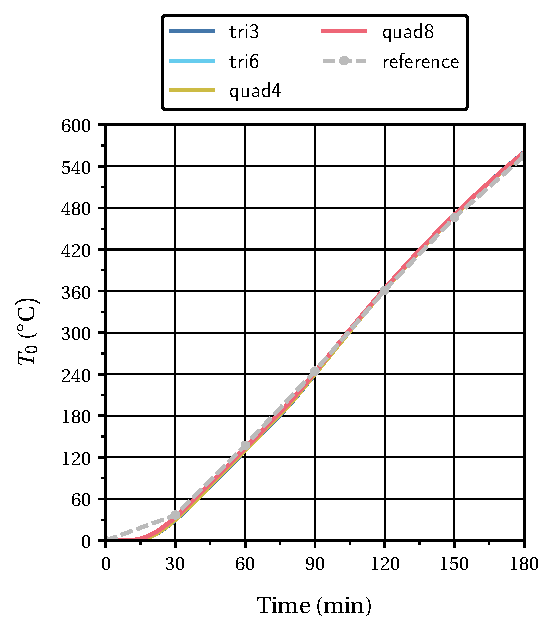
\includegraphics[width=0.5\columnwidth]{example_2_comparison_temp_ref_pt.pdf}
            \label{fig:example_2_comparison_temp_ref_pt}}
     \subfloat[][]{
    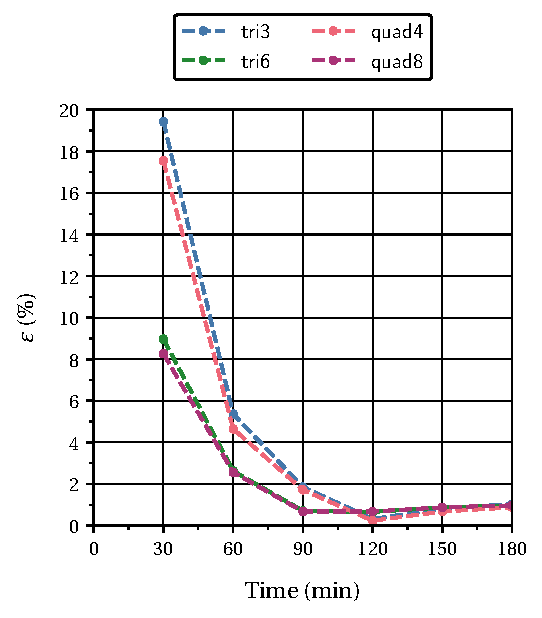
\includegraphics[width=0.5\columnwidth]{example_2_comparison_relative_error.pdf}
            \label{fig:example_2_comparison_relative_error}}
    \caption{Numerical results regarding the evolution of the temperature distribution for the validation example 2. (a) Temperature values at \(X\) as a function of time. (b) Relative error in percentage as function of time.}
    \label{fig:dim_example_2_comparison}
\end{figure}

\begin{figure}
   \centering
     \subfloat[][$t=\SI{30}{\minute}$]{ 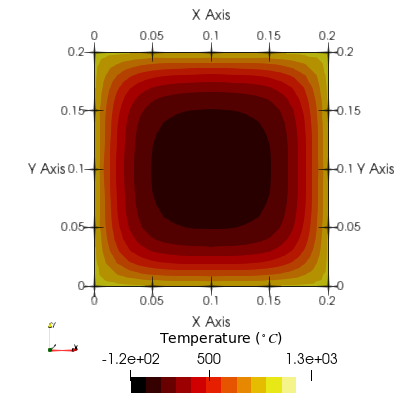
\includegraphics[width=0.5\columnwidth]{DIN_example_2_TRI3_t_30.png}
            \label{fig:DIN_example_2_TRI3_t_30}}
     \subfloat[][$t=\SI{90}{\minute}$]{ 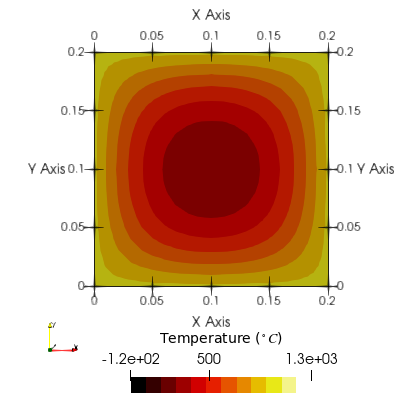
\includegraphics[width=0.5\columnwidth]{DIN_example_2_TRI3_t_90.png}
            \label{fig:DIN_example_2_TRI3_t_90}}\\
     \subfloat[][$t=\SI{120}{\minute}$]{
    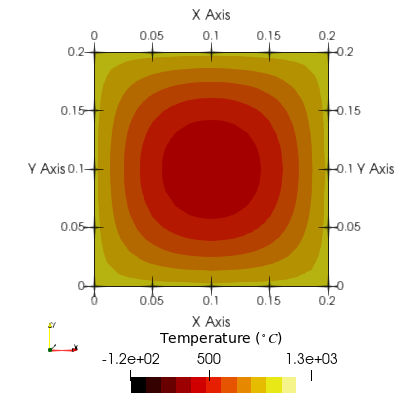
\includegraphics[width=0.5\columnwidth]{DIN_example_2_TRI3_t_120.png}
            \label{fig:DIN_example_2_TRI3_t_120}}
     \subfloat[][$t=\SI{180}{\minute}$]{
    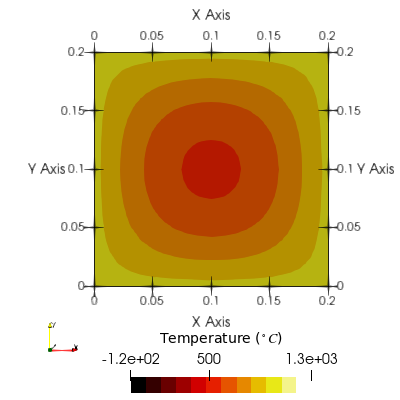
\includegraphics[width=0.5\columnwidth]{DIN_example_2_TRI3_t_180.png}
            \label{fig:DIN_example_2_TRI3_t_180}}
    \caption{Numerical results for the validation example 2 using a TRI3 mesh.}
    \label{fig:DIN_example_2_TRI3}
\end{figure}

\section{Validation example 3 - The Standard NAFEMS Benchmarks: linear thermo-elastic tests - Two dimensional heat transfer with convection}

\subsection{Description}

The geometry examined is a rectangular plate with width equal to \SI{0.6}{\meter} and length equal to \SI{1}{\meter}, as shown in Figure~\ref{fig:nafems_example_plate}.
A corresponding three-dimensional geometry is also considered with a thickness equal to \SI{1}{\meter}.
The boundary conditions considered are as follows: the left edge is assumed to be adiabatic.
At the lower edge the temperature is prescribed to be \SI{100}{\celsius} and along the upper and right edges there is heat transfer by convection and radiation.
The heat convection coefficient \(h\) is equal to \SI{70}{\watt\meter^{-2}\kelvin^{-1}}, and the ambient temperature is equal to \SI{0}{\celsius} (see Equation~\ref{eq:heat_convection}).
The initial temperature for the entire plate is \SI{0}{\celsius}.
The relevant properties of the material making up the plate are its conductivity \(k\), equal to \SI{52}{\watt\meter^{-1}\kelvin^{-1}}, its specific heat \(c_p\), equal to \SI{1}{\joule\kilo\gram^{-1}\kelvin^{-1}}, and its density \(\rho\), set equal to \SI{1}{\kilo\gram\meter^{-3}}.
Table~\ref{tab:nafems_example_description} summarizes all the information regarding initial and boundary conditions, geometry and material properties.
The expected temperature at E (see Figure~\ref{fig:nafems_example_plate}) is \SI{18.3}{\celsius}.


\begin{figure}
  \centering
  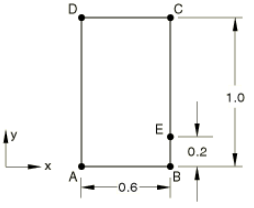
\includegraphics[width=0.55\textwidth]{nafems_example_plate.png}
  \caption{Geometry and boundary conditions considered in the validation example 3 \citep{NAFEMSbenchmarks}.}
\label{fig:nafems_example_plate}
\end{figure}

\begin{table}
  \centering
  \caption{Material properties, and initial and boundary conditions for validation example 3.}
  \label{tab:nafems_example_description}
  \begin{tabular}{lccS}
  \multicolumn{3}{c}{Material Properties} & {\vphantom{\Big |}Effective value}\\
  \hline\hline
  \vphantom{\Big |}Conductivity & \(k\) & (\si{\watt\meter^{-1}\kelvin^{-1}}) & 52\\
  \vphantom{\Big |}Specific heat & \(c_p\) & (\si{\joule\per\kilo\gram\per\kelvin}) & 1\\
  \vphantom{\Big |}Density & \(\rho\) & (\si{\kilo\gram\per\meter^{3}}) & 1\\
  \hline
  \multicolumn{3}{c}{Boundary Conditions\vphantom{\Big |}} & \\\hline
  \vphantom{\Big |}Dimension & \(h\) & (\si{\meter}) & 1\\
  \vphantom{\Big |}Dimension & \(b\) & (\si{\meter}) & 0.6\\
  \vphantom{\Big |}Thickness & \(t\) & (\si{\meter}) & 1\\
  Heat convection coefficient & \(h_c\) & (\si{\watt\per\meter^2\per\kelvin}) & 70\\
  \hline
  \multicolumn{3}{c}{Initial Conditions\vphantom{\Big |}} & \\\hline
  \vphantom{\Big |}Ambient temperature & \(T_\infty\) & (\si{\celsius}) & 100\\
  \vphantom{\Big |}Temperature in cross-section & \(T_0\) & (\si{\celsius}) & 0\\
  \hline
  \multicolumn{3}{c}{Reference value \vphantom{\Big |}} & \\\hline
  \vphantom{\Big |}Temperature \(T_0\) at point \(E\) & & (\si{\celsius}) & \\
  \hline\hline
  \end{tabular}
\end{table}

\subsection{Results}

The numerical solutions obtained using FEM are presented in Table~\ref{tab:nafems_example_comparison_table_2d} for two dimensions and in Table~\ref{tab:nafems_example_comparison_table_3d} for three-dimensions, as well as, the reference values and the corresponding relative difference.
It can be seen that that agreement between the numerical results and the reference solutions is acceptable.
It is below 1\% for all elements employed, except for the TETRA4 element.
There is no significant difference between the two integrators tested.
Figure~\ref{fig:NAFEMS_example_comparison} shows the temperature distribution obtained using TRI3 and TETRA10 elements, which is reasonable given the description of the problem.

\begin{table}
  \centering
  \caption{Reference and computed values for \(T_0\) concerning the validation example 3 in two-dimensions.}
\label{tab:nafems_example_comparison_table_2d}
  \begin{tabular}{c
  S[round-mode=places, round-precision=4]
  S[exponent-mode=scientific, round-mode=places, round-precision=2]}
  \vphantom{\Big |}Element & {\makecell{Temperature \(T_0\)\\at \(E\) \si{\celsius} } } & {\makecell{Relative\\ difference \(\varepsilon\) (\(\%\))}} \\
  \hline
  \multicolumn{3}{l}{\vphantom{\Big |}Alpha integrator (\(\rho=1\))}\\
  \hline
    TRI3 & 18.189045 & 0.6065573770491839\\
    TRI6 & 18.255251 & 0.24426229508198033\\
    QUAD4 & 18.228554 & 0.39016393442623263\\
    QUAD8 & 18.253191 & 0.2557377049180386\\
  \hline
  \multicolumn{3}{l}{\vphantom{\Big |}Quasi static integrator}\\
  \hline
    TRI3 & 18.189476 & 0.6038251366120318\\
    TRI6 & 18.254831 & 0.24699453551913246\\
    QUAD4 & 18.228132 & 0.39289617486338475\\
    QUAD8 & 18.253622 & 0.2535519125683169\\
    \hline\hline
  \end{tabular}
\end{table}

\begin{table}
  \centering
  \caption{Reference and computed values for \(T_0\) concerning the validation example 3 in three-dimensions.}
\label{tab:nafems_example_comparison_table_3d}
  \begin{tabular}{c
  S[round-mode=places, round-precision=4]
  S[exponent-mode=scientific, round-mode=places, round-precision=2]}
  \vphantom{\Big |}Element & {\makecell{Temperature \(T_0\)\\at \(E\) \si{\celsius} } } & {\makecell{Relative\\ difference \(\varepsilon\) (\(\%\))}} \\
  \hline
  \multicolumn{3}{l}{\vphantom{\Big |}Alpha integrator (\(\rho=1\))}\\
  \hline
    TETRA4 & 17.950129 & 1.9118633879781435\\
    TETRA10 & 18.255579 & 0.2427377049180318\\
  \hline
  \multicolumn{3}{l}{\vphantom{\Big |}Quasi static integrator}\\
  \hline
    TETRA4 & 17.949707 & 1.9141693989071074\\
    TETRA10 & 18.254831 & 0.2468251366120292\\
    \hline\hline
  \end{tabular}
\end{table}

\begin{figure}
   \centering
   \subfloat[][]{ 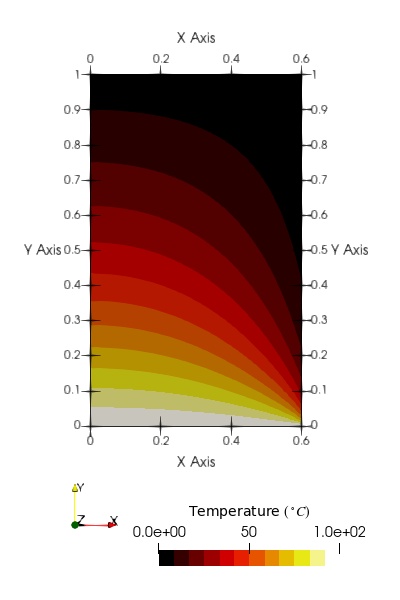
\includegraphics[width=0.5\columnwidth]{tri3_alpha.png}
   \label{fig:tri3_alpha}}
   \subfloat[][]{ 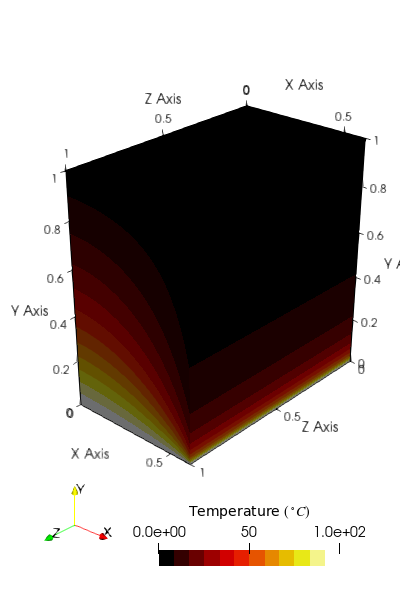
\includegraphics[width=0.5\columnwidth]{tetra10_alpha.png}
   \label{fig:tetra10_alpha}}
  \caption{Temperature distribution concercing the validation example 3: (a) in two-dimensions (TRI6) (b) in three-dimensions (TETRA4).}
\label{fig:NAFEMS_example_comparison}
\end{figure}
